% !TeX root = ../technical_paper.tex
\section{软件设计与流程}

\subsection{软件总体架构}

系统软件采用分层架构，自下而上包括驱动层、采样与保护层、控制算法层、能量管理层和通信交互层。驱动层负责 ADC、PWM、定时器、通信接口和 GPIO 初始化；采样与保护层完成数据滤波、量纲转换、阈值判断和故障锁存；控制算法层主要运行 SOC 估算、CC/CV 充电控制、状态机管理和保护策略等功能。针对 MPPT、母线稳压、交流输出控制等功能，已完成软件框架预留，将在后续阶段进一步完善；能量管理层根据光伏功率、负载功率、SOC 和故障状态选择工作模式；通信交互层完成 MCU 间数据同步和无线监控。

GD32G553 主控工程划分为四层：
\begin{itemize}[leftmargin=*,itemsep=0.5ex]
  \item \textbf{HAL层}：对 ADC、HRTIMER、CAN、UART、GPIO 等外设进行统一抽象，屏蔽底层硬件差异
  \item \textbf{Protocol层}：完成 CAN FD 帧解析与 UART AA55 帧封装，实现标准协议与自定义协议的转换
  \item \textbf{Middleware层}：发布/订阅式数据总线，解耦数据生产者与消费者，支持模块间零耦合通信
  \item \textbf{APP层}：统一调度器组织各模块运行，包括 BMS 数据转发、心跳帧输出、CC/CV 充电控制和 G2S 状态管理等
\end{itemize}

\begin{figure}[htbp]
  \centering
  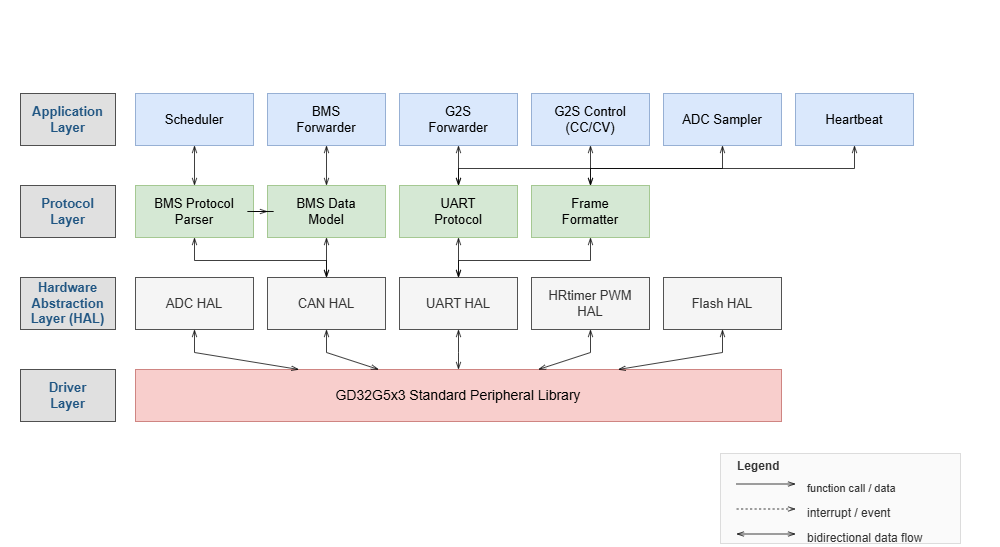
\includegraphics[width=0.82\textwidth]{images/流程图架构图/GD32G553软件架构.drawio.png}
  \caption{GD32G553主控软件四层架构}
  \label{fig:software_arch}
  \vspace{0.2em}
  {\small 资料来源：作者绘制。}
\end{figure}

系统上电后依次完成外设初始化、自检、BMS 通信检测、无线模块连接。初始化完成后进入主循环，按固定周期执行采样、状态判断、通信处理和控制输出。主控调度器采用时间片轮转机制，各模块按预设周期独立运行：BMS 数据解析每 100 ms 执行一次，心跳帧输出每 1000 ms 执行一次，ADC 采样每 10 ms 触发一次 DMA 传输。

\subsection{BMS产品状态机}

GD32C113 BMS 工程采用产品状态机管理运行流程，主要包含三种状态：

\textbf{（1）INIT\_FAIL状态}

系统上电后进入初始化阶段，依次完成：
\begin{enumerate}[label=\arabic*),leftmargin=*,itemsep=0.3ex]
  \item 板级初始化（时钟、GPIO、通信接口、看门狗配置）
  \item AFE最小唤醒（GD30BM2016寄存器配置、16S配置、CCGain设置）
  \item FET通路关闭、均衡清零
  \item 完整AFE配置：保护阈值装载、温度传感器类型配置、ADC校准
\end{enumerate}

若初始化过程中AFE通信失败、配置异常或自检不通过，系统进入INIT\_FAIL状态，保持FET关闭并上报初始化故障。看门狗定时器在初始化阶段即启动，若初始化超时未进入正常状态，则触发系统复位。

\textbf{（2）RUN状态}

当首次测量有效、无严重故障且电芯状态正常时，系统进入RUN状态。每个控制周期（约 100 ms）依次执行：
\begin{enumerate}[label=\arabic*),leftmargin=*,itemsep=0.3ex]
  \item 测量模块：通过I2C读取AFE电压、电流、温度数据，进行数据有效性校验
  \item 保护模块：过压（COV）、欠压（CUV）、过流（OCD/OCC）、短路（SCD）、过温（OT）、欠温（UT）判断
  \item SOC模块：OCV种子初始化结合安时积分进行SOC估算
  \item 均衡模块：判断单体电压差，执行被动均衡（支持逐节均衡和最大导通时间保护）
  \item FET模块：根据保护状态和充放电允许条件更新CHG/DSG/PCHG/PDSG策略
  \item 通信模块：组织CAN FD遥测帧（0x300--0x310）并周期性发送
\end{enumerate}

% TODO: 插入BMS状态机状态转移图
\begin{figure}[htbp]
  \centering
  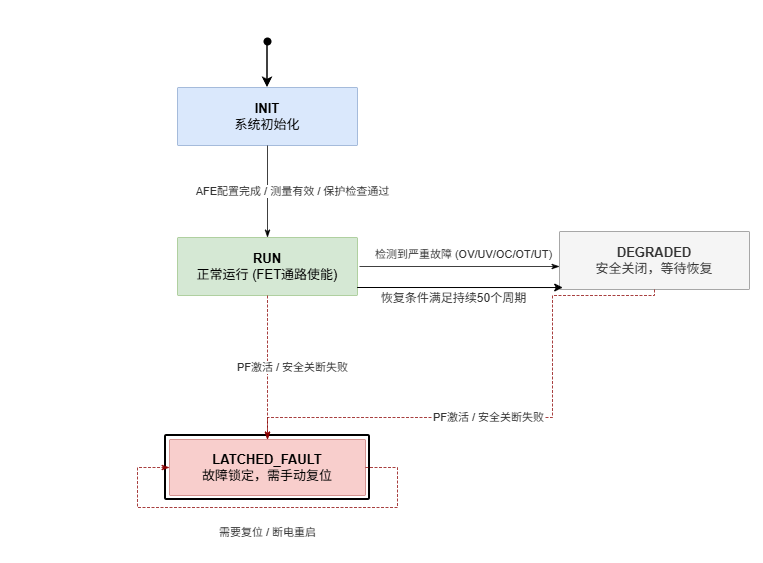
\includegraphics[width=0.78\textwidth]{images/流程图架构图/BMS运行时状态机.drawio.png}
  \caption{BMS产品状态机}
  \label{fig:bms_state_machine}
  \vspace{0.2em}
  {\small 资料来源：作者绘制。}
\end{figure}

\textbf{（3）DEGRADED状态}

若运行过程中出现以下任一情况，系统立即进入DEGRADED状态：
\begin{itemize}[leftmargin=*,itemsep=0.3ex]
  \item AFE读取失败或I2C通信超时（连续3次通信失败）
  \item 保护项触发（COV/CUV/OCD/SCD/OT/UT任一项达到阈值）
  \item FET应用失败（路径检测不通过）
  \item 严重安全异常或看门狗超时
\end{itemize}

进入DEGRADED后，系统执行均衡抑制和FET全关断，停止充放电通路。对于可恢复故障，待异常条件消除后重新评估是否返回RUN状态；对于锁存故障，需通过上位机下发清故障命令或重新上电恢复。

\subsubsection{安全保护分级处理}

BMS安全保护按照故障严重程度分为三级处理机制：

\textbf{（1）预警级}
当检测到温度轻微异常或电压接近阈值时，系统记录告警日志并通过CAN上报，不执行关断操作，持续监测趋势变化。

\textbf{（2）限制级}
当保护项触发但尚未达到危险阈值时（如轻微过压），系统限制充放电电流或暂停充电，同时维持通信和采样功能。

\textbf{（3）关断级}
当出现严重过压、欠压、过流、短路或过温等危险故障时，系统立即关闭所有FET通路，进入DEGRADED状态，等待故障清除或人工干预。

\subsection{SOC估算算法}

\subsubsection{OCV-库仑混合估算策略}

磷酸铁锂电池在 $30\%$--$80\%$ SOC 区间的 OCV 曲线较为平坦，单纯依靠电压判断 SOC 误差较大；而安时积分法又存在累计漂移和初值依赖问题。本作品采用 OCV 种子自适应初始化结合动态库仑计数的混合策略，兼顾两种方法的优点。

系统通过离线实验标定 OCV-SOC 曲线并以查表形式存储于 MCU Flash。标定采用小电流（C/20）恒流充放电，每个 SOC 点静置足够长时间后记录稳定开路电压。由于平坦区间的限制，采用分段策略：低 SOC（$<30\%$）和高 SOC（$>80\%$）区间直接通过 OCV 查表获得准确初值；中间区间主要依赖安时积分跟踪。

安时积分法离散化形式为

\[
\mathrm{SOC}_k=\mathrm{SOC}_{k-1}-\frac{\eta\cdot I_k\cdot\Delta t}{C_{\mathrm{nom}}}\times100\%,
\]

其中 $C_{\mathrm{nom}}$ 为额定容量，$\eta$ 为充放电效率，$I_k$ 为实时电流。系统对电流信号进行滑动平均滤波，并设置最小累计阈值（电流小于 $50\,\mathrm{mA}$ 时暂停积分，视为静置状态），以减小采样噪声影响。

\subsubsection{混合策略实现流程}

本作品采用OCV种子自适应初始化结合动态库仑计数的混合估算策略，算法流程如下：

\begin{enumerate}[label=\arabic*),leftmargin=*,itemsep=0.3ex]
  \item \textbf{上电初始化}：系统上电后，若电池已静置超过30分钟，直接通过OCV查表获得SOC初值；若未满足静置条件，则使用上次关机前保存的SOC值作为初值。
  \item \textbf{运行阶段}：正常运行时以安时积分法为主进行SOC动态跟踪，每100 ms更新一次累计值。
  \item \textbf{OCV修正}：当系统检测到电池进入静置状态（电流持续低于阈值超过5分钟），触发OCV修正流程。读取当前OCV并通过查表获得参考SOC，若与当前积分SOC偏差超过3\%，则以OCV查表值为准进行修正。
  \item \textbf{满充校准}：当充电电压达到单体满充电压（$3.65\,\mathrm{V}$）且充电电流降至截止电流以下时，将SOC强制校准为100\%。
  \item \textbf{深度放电校准}：当任一单体电压降至放电截止电压（$2.5\,\mathrm{V}$）时，将SOC强制校准为0\%。
\end{enumerate}

该混合策略兼顾了OCV法在稳态下的准确性和库仑计数法在动态过程中的连续性，通过定期的OCV修正消除了累计漂移，使SOC估算误差控制在$5\%$以内。

% TODO: 插入SOC估算流程图
\begin{figure}[htbp]
  \centering
  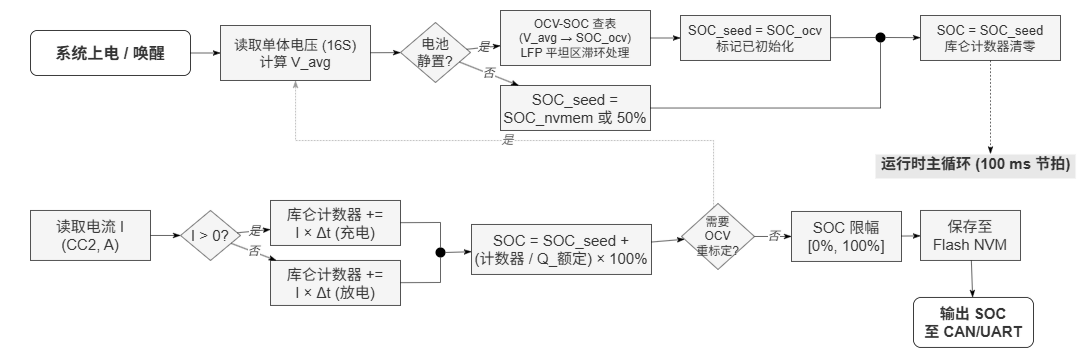
\includegraphics[width=0.95\textwidth]{images/流程图架构图/SOC估计算法流程图.drawio.png}
  \caption{OCV-库仑混合SOC估算流程}
  \label{fig:soc_flowchart}
  \vspace{0.2em}
  {\small 资料来源：作者绘制。}
\end{figure}

\subsection{电池均衡控制}

\subsubsection{被动均衡原理}

本系统采用被动均衡方案，每节电池对应一路均衡支路。当某一节电池电压高于均衡阈值时，BMS控制对应MOSFET导通，使该单体通过放电电阻释放部分能量，从而逐步减小单体间电压差。

\subsubsection{基于电压差的均衡策略}

均衡策略以单体电压差为判断依据。每个控制周期内，BMS计算16节电池中的最高电压 $V_{\max}$ 和最低电压 $V_{\min}$，当满足以下条件时触发均衡：

\begin{enumerate}[label=\arabic*),leftmargin=*,itemsep=0.3ex]
  \item $V_{\max}-V_{\min}>\Delta V_{\mathrm{th}}$（典型值为 $30\,\mathrm{mV}$）
  \item 待均衡单体电压高于平均电压
  \item 系统处于充电状态或静置状态（放电期间禁止均衡）
  \item 当前无保护故障
\end{enumerate}

均衡采用逐节轮询方式，每次最多同时均衡4节单体，以避免均衡功耗过大导致BMS板温升过高。

\subsubsection{均衡安全保护}

为防止均衡支路长时间导通导致过热，系统设置了以下保护机制：
\begin{itemize}[leftmargin=*,itemsep=0.3ex]
  \item \textbf{最大导通时间限制}：单路均衡连续导通时间不超过30分钟，超时自动关闭
  \item \textbf{温度限制}：当BMS板温度超过$60\,\mathrm{°C}$时，暂停所有均衡操作
  \item \textbf{电压下限保护}：均衡单体电压低于$3.0\,\mathrm{V}$时停止该路均衡
\end{itemize}

\subsection{CC/CV充电闭环控制}

主控侧实现了恒流恒压（CC/CV）充电闭环控制策略，支持三端口储能场景下的电池充电管理。

\subsubsection{CC/CV控制策略与状态转换}

充电过程分为三个阶段，状态转换关系如图~\ref{fig:cc_cv_state_machine}所示：

\begin{enumerate}[label=\arabic*),leftmargin=*,itemsep=0.3ex]
  \item \textbf{CC阶段}：当电池SOC低于设定阈值且BMS允许充电时，系统进入恒流充电状态。充电电流由BMS根据电池温度和状态动态计算允许值，主控以该允许值作为电流环设定值，电池电压持续上升。
  \item \textbf{CV阶段}：当任一单体电压达到设定恒压阈值（如$3.55\,\mathrm{V}$）时，状态由CC切换至CV。系统维持电压恒定，充电电流自然衰减。
  \item \textbf{FULL阶段}：当充电电流降至截止电流（如$0.05\,\mathrm{C}$）时，状态切换为FULL，停止充电并将SOC强制校准为100\%。
\end{enumerate}

状态转换条件：
\begin{itemize}[leftmargin=*,itemsep=0.3ex]
  \item CC $\rightarrow$ CV：最高单体电压 $\ge V_{\mathrm{cv\_th}}$
  \item CV $\rightarrow$ FULL：充电电流 $\le I_{\mathrm{cutoff}}$
  \item 任意状态 $\rightarrow$ STOP：BMS禁止充电或保护触发
\end{itemize}

\subsubsection{PI控制器参数整定}

电流环和电压环均采用PI控制器，离散形式为

\[
u(k)=K_p\cdot e(k)+K_i\cdot\sum_{i=0}^{k}e(i),
\]

其中 $e(k)$ 为设定值与反馈值的偏差，$K_p$ 和 $K_i$ 分别为比例和积分系数。控制器输出经限幅后作为PWM占空比指令，通过HRTIMER输出至功率级。

参数整定采用试凑法结合仿真验证，在确保稳定性的前提下尽量提高响应速度。电流环带宽设置为开关频率的1/10，电压环带宽低于电流环以避免环间耦合。

\begin{figure}[htbp]
  \centering
  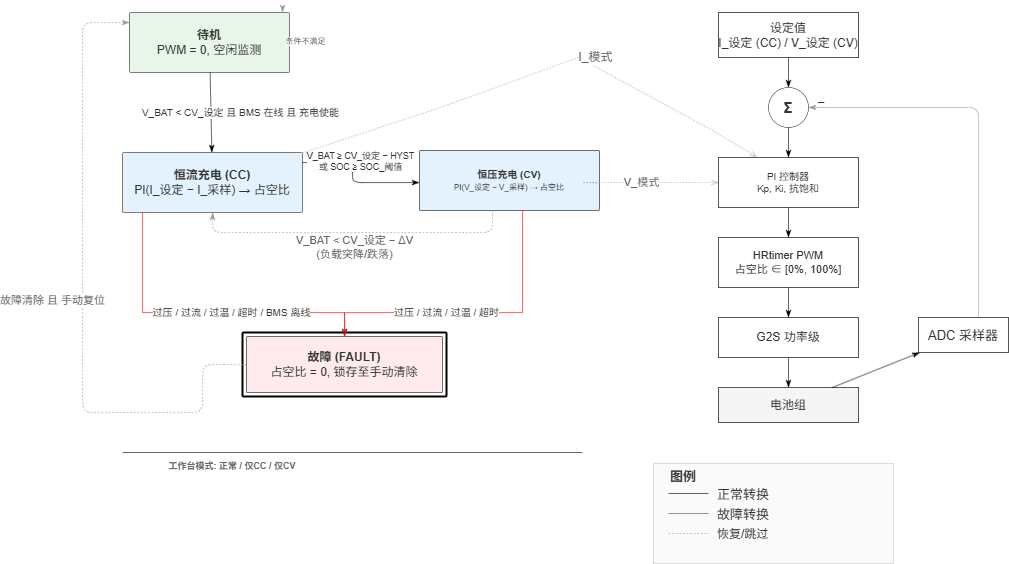
\includegraphics[width=0.82\textwidth]{images/流程图架构图/CCCV充电状态机.png}
  \caption{CC/CV充电状态机}
  \label{fig:cc_cv_state_machine}
  \vspace{0.2em}
  {\small 资料来源：作者绘制。}
\end{figure}

\subsection{多MCU通信协议}

\subsubsection{CAN FD遥测协议（BMS → 主控）}

BMS通过CAN FD周期性发送遥测帧，通信速率为500 kbps（仲裁段）/ 2 Mbps（数据段）。关键报文定义如表~\ref{tab:can_protocol}所示。

% TODO: 补充实际CAN帧字段定义
\begin{table}[htbp]
  \centering
  \caption{BMS CAN FD关键报文定义}
  \label{tab:can_protocol}
  \begin{tabular}{@{}clp{8.5cm}@{}}
    \toprule
    \textbf{帧ID} & \textbf{名称} & \textbf{内容说明} \\
    \midrule
    0x300 & 电池总压电流 & 电池包总电压 (0.01~V/bit)、总电流 (0.01~A/bit)、SOC (1\%/bit) \\
    0x301 & 单体电压 1--8 & 电芯 1 至电芯 8 电压 (0.001~V/bit) \\
    0x302 & 单体电压 9--16 & 电芯 9 至电芯 16 电压 (0.001~V/bit) \\
    0x303 & 温度与状态 & 温度 (0.1~$^\circ$C/bit)、均衡状态位图、故障标志 \\
    0x310 & 保护状态 & FET 状态、允许充放电标志、DEGRADED 状态码 \\
    \bottomrule
  \end{tabular}
\end{table}
\vspace{-0.3em}
{\small 资料来源：作者根据 GD30BM2016 AFE 数据手册及实际通信协议整理。}

每个遥测帧均包含滚动计数器（Rolling Counter）和校验字段，用于接收端检测丢帧和数据完整性。主控在接收到CAN帧后，首先校验帧ID和长度，然后解析数据并更新内部BMS数据模型。

\subsubsection{UART数据帧协议（主控 ↔ 无线模块）}

主控与GD32VW553之间采用固定格式的UART数据帧，波特率115200，帧结构如表~\ref{tab:uart_protocol}所示。

\begin{table}[htbp]
  \centering
  \caption{UART数据帧格式}
  \label{tab:uart_protocol}
  \begin{tabular}{@{}cll@{}}
    \toprule
    \textbf{字段} & \textbf{长度} & \textbf{说明} \\
    \midrule
    帧头     & 2~字节 & 固定为 0xAA~0x55 \\
    命令字   & 1~字节 & 0x01=BMS数据、0x02=心跳帧、0x04=G2S数据、0x81=命令响应 \\
    数据长度 & 1~字节 & 后续数据区字节数 $N$ \\
    数据区   & $N$~字节 & 有效载荷（具体格式由命令字定义） \\
    校验和   & 1~字节 & 累加和校验（帧头+命令字+数据长度+数据区） \\
    \bottomrule
  \end{tabular}
\end{table}
\vspace{-0.3em}
{\small 资料来源：作者根据主控与无线模块实际通信协议整理。}

无线模块采用状态机方式解析AA55帧：接收过程中依次匹配帧头、读取命令字和数据长度、接收数据区、校验校验和。若任一环节出错，则丢弃当前帧并复位解析器，等待下一帧帧头。

\subsection{无线通信与云端监控}

\subsubsection{MQTT客户端设计}

GD32VW553无线模块运行FreeRTOS，通过WiFi STA模式连接路由器后，启动MQTT客户端与云端Broker建立连接。MQTT通信采用以下Topic设计：
\begin{itemize}[leftmargin=*,itemsep=0.3ex]
  \item \texttt{device/\{id\}/telemetry}：设备周期性上报遥测数据（JSON格式，含电压、电流、SOC、温度、模式等）
  \item \texttt{device/\{id\}/command}：云端下发控制命令（模式切换、参数配置等）
  \item \texttt{device/\{id\}/response}：设备对命令的响应ACK
\end{itemize}

遥测数据上报周期为1--5秒可调，QoS等级为1（至少送达一次），确保关键状态信息不丢失。

\subsubsection{Web监控服务器}

为便于现场调试和演示，开发了基于Python的轻量级Web监控服务器。服务器架构采用MQTT桥接 + HTTP服务器 + Server-Sent Events（SSE）三层设计：
\begin{enumerate}[label=\arabic*),leftmargin=*,itemsep=0.3ex]
  \item MQTT桥接模块订阅设备遥测Topic，接收实时数据并缓存至内存数据库
  \item HTTP服务器提供静态页面服务，前端界面通过JavaScript建立SSE连接
  \item SSE模块将最新遥测数据以text/event-stream格式实时推送至浏览器，实现无需刷新的实时数据可视化
\end{enumerate}

该方案无需安装专用App或客户端，任何支持浏览器的设备（PC、平板、手机）均可通过访问服务器IP查看系统运行状态，显著降低了远程监控部署成本。

% TODO: 插入Web服务器架构图
\begin{figure}[htbp]
  \centering
  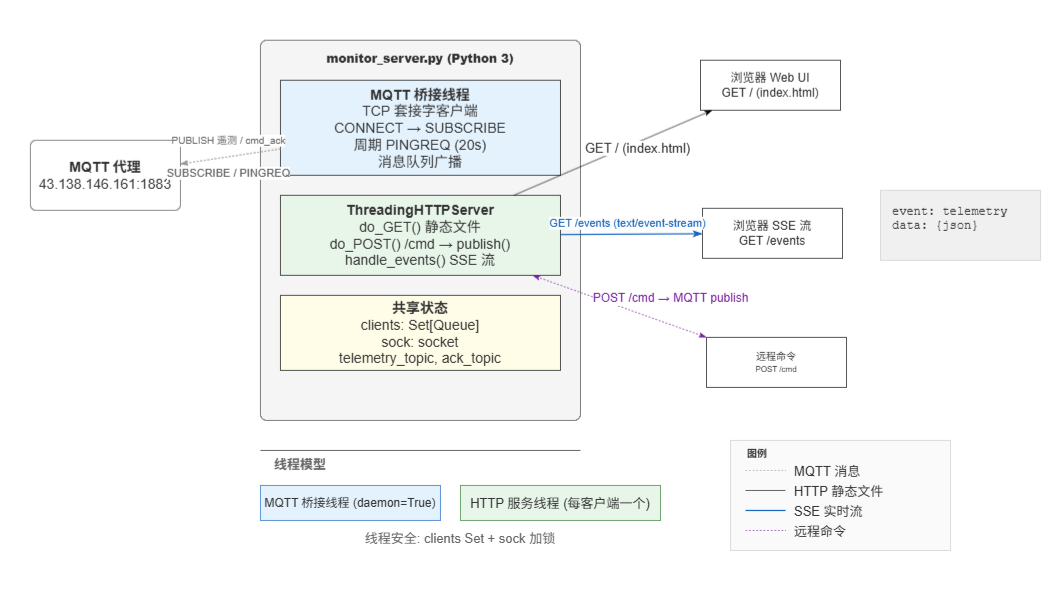
\includegraphics[width=0.95\textwidth]{images/流程图架构图/Python网络监控服务器架构.drawio.png}
  \caption{Web监控服务器架构}
  \label{fig:web_server_arch}
  \vspace{0.2em}
  {\small 资料来源：作者绘制。}
\end{figure}

\subsection{后续控制策略规划}

基于当前已搭建的控制平台和三端口功率变换硬件基础，后续阶段计划实现以下控制策略：

\textbf{（1）前级三端口能量管理。} 在已完成 PV$\rightarrow$Battery 充电功能验证的基础上，后续将围绕光伏功率 $P_{\mathrm{pv}}$、负载功率 $P_{\mathrm{load}}$、电池 SOC 和故障状态，实现光伏独立供电、光伏充电、光伏与电池联合供电以及电池离网供电等多模式能量调度。MPPT 控制拟采用扰动观察法，充电电流受 BMS CC/CV 限值约束。

\textbf{（2）后级交流变换控制。} 离网模式下，交流变换器生成 50 Hz 正弦参考，通过电压外环和电流内环控制全桥 PWM，配合 LC 滤波器实现交流输出。前后级之间通过母线电压协调，减少负载阶跃引起的母线过冲和输出波形畸变。

\subsection{多 MCU 协同控制策略}

三颗 MCU 之间采用主从协同关系。GD32G553 是功率控制主节点，周期性接收 BMS 状态和无线配置参数，并向无线模块发送运行数据。GD32C113 是电池安全节点，向主控提供 SOC、允许充电电流、允许放电电流和故障状态。GD32VW553 是通信节点，负责将用户配置转换为主控可识别的参数命令。

若主控在设定时间内未收到 BMS 心跳（约 300 ms），则进入电池通信异常状态，限制充放电功率或停机保护。该超时机制确保了在 BMS 失联时主控能够及时采取安全措施。

\begin{table}[htbp]
  \centering
  \caption{MCU间关键交互数据}
  \label{tab:mcu_data}
  \begin{tabular}{@{}lp{5.2cm}p{6.8cm}@{}}
    \toprule
    \textbf{数据方向} & \textbf{数据内容} & \textbf{用途} \\
    \midrule
    BMS $\rightarrow$ 主控     & SOC、单体极值、温度、充放电允许电流、故障码 & 决定能量调度、限流和保护状态 \\
    主控 $\rightarrow$ BMS     & 工作模式、端口电流、电池功率、系统故障状态 & 辅助 BMS 判断系统级风险 \\
    主控 $\rightarrow$ 无线模块 & 电压、电流、功率、SOC、模式、故障码 & 状态显示、日志记录和远程监控 \\
    无线模块 $\rightarrow$ 主控 & 目标模式、限值参数、复位/清故障命令 & 用户配置和运维控制 \\
    \bottomrule
  \end{tabular}
\end{table}
\vspace{-0.3em}
{\small 资料来源：作者根据系统多 MCU 协同架构整理。}
